%!TEX root = ../document.tex
\chapter{Grundlagen} \label{chp:Grundlagen}  
In den folgenden Abschnitten werden eine Reihe von Begriffen und Verfahren genutzt, die hier eingeführt werden sollen.     
Dies ermöglicht dem Leser die Beantwortung der Fragestellungen aus Abschnitt \ref{chp:Loesungsansatz} nachzuvollziehen.    
 
Zunächst werden einige geografische Grundbegriffe eingeführt. 

 
Zum Schluss wird die genutzte Datenbasis und der Einfluss der von Twitter genutzten Sampling-Strategie vorgestellt und erläutert.

\newpage

	\section{Geografische Grundlagen und Begriffe}
	
		In diesem Kapitel sollen geografische Grundbegriffe erläutert werden. 
		Einige geografische Begriffe werden in verschiedenen wissenschaftlichen Bereichen unterschiedlich genutzt und teilweise widersprüchlich definiert. 
		Um Missverständnissen vorzubeugen wird hier definiert was in der vorliegenden Arbeit unter den einzelnen Begriffen zu verstehen ist.
		Eine Reihe von Begriffen wird selbst definiert um bestimmte Sachverhalte im Kontext dieser Arbeit klarer ausdrücken zu können. 

		\subsection{Geografische Koordinaten}
			
			Geografische Koordinaten bestehen aus zwei Werten, einem Wert für den sogenannten Längengrad und einem Wert für den sogenannten Breitengrad.
			Mit diesen zwei Werten kann eine Position auf dem Globus exakt bestimmt werden.  
			
			Die Längen- und Breitengrade beschreiben ein imaginäres Netz auf dem Globus. 
			Dabei ziehen sich die Breitengrade wie ein Gürtel um den Globus.
			Der Breitengrad mit dem Wert 0 verläuft entlang des Äquators.

			Die Längengrade hingegen verlaufen vom Nord- zum Südpol. 
			Vertikal des Globus verläuft keine natürliche Marke. 
			Der Längengrad mit dem Wert 0 wurde deshalb 1884 durch ein Konsortium festgelegt.
			Die Längengrade werden auch als Meridiane bezeichnet.
			
			Die Werte liegen im IT-Umfeld meist als Fließkommazahlen vor und beschreiben jeweils einen Winkel.
			In Abbildung \ref{img:lnglat}, auf der linken Seite, sind die Längen- und Breitengrade auf einem Globus aufgetragen.

		\subsection{Geodätisches Referenzsystem} 
			
			Ein geodätisches Referenzsystem dient als einheitliche Grundlage zur Angabe einer Position auf dem Globus. 

			Es wird ein kartesisches Rechtssystem mit definierter Lage und Ausrichtung festgelegt.
			Die Lage und Ausrichtung erfolgt relativ zur Erde. 
			Der Ursprung des Koordinatensystems liegt im Zentrum des Globus, meist im Masseschwerpunkt der Erde.
			Die Z-Achse zeigt dabei in Richtung Nordpol und die X-Achse in Richtung 0 Grad Länge und 0 Grad Breite. 
			Mit diesen zwei Werten ist die Lage eines kartesischen Rechtssystem eindeutig definiert.
			In Abbildung \ref{img:lnglat}, auf der rechten Seite, ist die Lage des kartesischen Koordinatensystems dargestellt.

			In diesem Koordinatensystem sind zusätzlich Referenzpunkte festgelegt.
			Diese Referenzpunkte werden benötigt um einen Referenzellipsoid zu verankern. 
			Auf diesem Ellipsoid sind ebenfalls definierte Referenzpunkte festgelegt, die mit den Referenzpunkten im Koordinatensystem zur Deckung gebracht werden.
			Der Referenzellipsoid soll eine möglichst genaue Approximation der Erde darstellen und diese im geodätischen Referenzsystem repräsentieren. 
			Ein Punkt auf diesem Ellipsoid entspricht damit einem Punkt auf der Erde.

			Mit diesen Komponenten kann nun ein Punkt auf dem Ellipsoid eindeutig bestimmt werden.
			Der Längen- und Breitengrad eines Punktes P auf dem Ellipsoid lässt sich folgendermaßen bestimmen:

			Durch den Punkt P auf dem Ellipsoid und den Ursprung z des Koordinatensystems wird eine Gerade g gezogen. 
			Der Wert für den Breitengrad ist nun der Winkel $\phi$ zwischen g und der Äquatorebene.
			Nun wird der Punkt P auf die Äquatorebene projiziert.
			Zwischen z und dem projizierten Punkt Q kann nun wiederum eine Gerade h gezogen werden.
			Der Wert für den Längengrad ist der Winkel $\lambda$ zwischen der X-Achse und der Gerade h. 
			In Abbildung \ref{img:lnglat}, auf der rechten Seite, ist dies dargestellt.
			Durch eine Projektion der Punkte auf den Ellipsoid können diese Punkte beispielsweise auf einer Karte dargestellt werden.
			Einfach gesprochen wird der Referenzellipsoid "'aufgeklappt"'. 
			Durch die Referenzpunkte kann dann eine Karte auf dem Ellipsoid abgebildet werden.
			\footnote{Vergleiche Geoinformatik Lexikon der Universität Rostock (abgerufen Juli 2014): http://www.geoinformatik.uni-rostock.de/lexikon.asp \\ Vorlesungen zur Geo-Informatik von Prof. Dr.-Ing. Ralf Bill (abgerufen Juli 2014): http://www.geoinformatik.uni-rostock.de/vorlesungsthem.asp \label{ft:geoinfolex}  Juli 2014}

			Heutzutage ist das Referenzsystem WGS84 weit verbreitet.

			\begin{figure}[h!]
			\begin{center}
				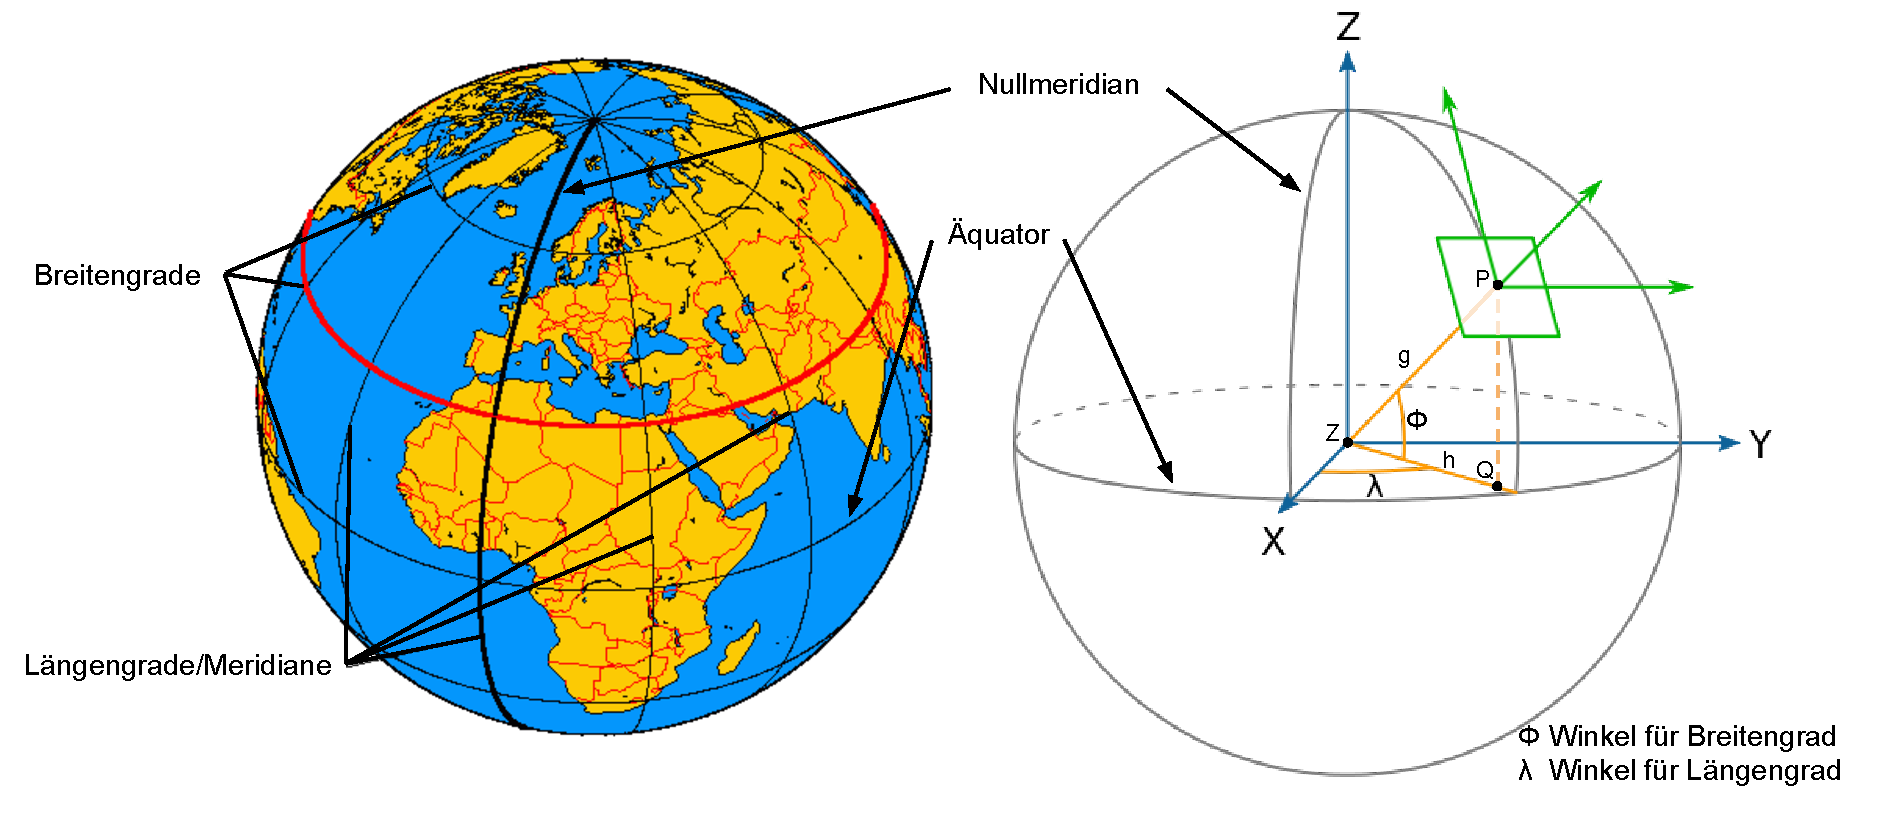
\includegraphics[scale=0.5]{globuseMitLngLat.pdf}
				\caption{Längen- und Breitengrade}
				\label{img:lnglat}
			\end{center}
			\end{figure}	
			%vgl. http://de.wikipedia.org/wiki/Meridian_(Geographie)#mediaviewer/Datei:Meridian-International.PNG
			%vgl. http://en.wikipedia.org/wiki/Geodetic_datum#mediaviewer/File:ECEF_ENU_Longitude_Latitude_relationships.svg

		\subsection{Georeferenz} 
			
			Eine Georeferenz (engl. Spatial Reference) wird auch als Raumbezug bezeichnet. 
			Ist einem Datensatz, einem Datum oder einem Objekt eine geografische Lage oder Position zugeordnet so wird diese als Georeferenz bezeichnet.1 
			Eine Georeferenz kann auf verschiedene Arten und mit unterschiedlicher Genauigkeit angegeben werden.
			Dies hängt von den Anforderungen ab, die an die Georeferenz gestellt werden. 
			Beispielsweise stellen die in Kapitel \ref{chp:Einleitung} erwähnten Anwendungen unterschiedliche Anforderungen an die Genauigkeit der Georeferenz. \footref{ft:geoinfolex} 
			
			Die Georeferenz lässt sich bezüglich der Genauigkeit weiter unterteilen in: 
		
			\begin{description}

	 			\item[Direkte Georeferenz (direkter Raumbezug)] 
	 				
	 				Unter einer direkten Georeferenz versteht man die Angabe einer konkreten Koordinate bezüglich eines geeigneten geodätischen Referenzsystems. \footref{ft:geoinfolex} 

	 			\item[Indirekte Georeferenz (indirekter Raumbezug) ] 
	 				
	 				Unter indirektem Raumbezug werden alle Angaben verstanden die eine ungenaue Position bezüglich eines beliebigen Referenzysystems bestimmen.
		 			Ungenau ist in dem Sinne zu verstehen, dass die Angabe der Position auch eine Fläche beschreiben kann.
		 			Zusätzlich muss das gewählte Referenzsystem nicht zwingenderweise unveränderlich sein.   
		 			Beispiele für die Angabe eines indirekten Raumbezugs wären Länder, Adressen, Postleitzahlen oder auch Telefonvorwahlen. 
		 			Alle diese Angaben, mit Ausnahme der Adresse, definieren eine geografische Fläche. 
		 			Diese Fläche ist nicht zwingenderweise klar abzugrenzen. \footref{ft:geoinfolex} 

			\end{description}

		\subsection{Geografische Objekte}
			
			Ein geografisches Objekt ist ein Objekt der Realwelt dessen Position durch eine Georeferenz bestimmt werden kann. 
			Die EN ISO 19110:2005 Norm beschreibt ein geografisches Objekt folgendermaßen: 

			"'Geografische Objekte sind Erscheinungen der realen Welt, die einen Bezug zur Erde (Raumbezug) haben..."' \cite{ISO19110:2005}.

			Es wird insbesondere nicht festgelegt ob es sich dabei um eine direkte oder eine indirekte Georeferenz handelt.
			Beispiele für geografische Objekte sind: Städte, Länder, Häuser oder auch Fahrzeuge.
			Insbesondere sind auch Menschen geographische Objekte, da sie zu jeder Zeit einen Bezug zur Erde haben.

		\subsection{Toponyme}  
			
			Toponyme sollen hier Namen für geografische Objekte mit unveränderlicher geografischer Position sein.
			Beispiele für Toponyme sind Städtenamen, Ländernamen oder Landschaftsnamen.  
			Ein Toponym muss nicht eindeutig sein. 

		\subsection{Geografische Position}
		
			Unter einer geografischen Position soll hier eine Position auf dem Globus verstanden werden deren Wert durch geografische Koordinaten angegeben wird.

		\subsection{Geografische Region} 
			
			Unter einer geografischen Region werden hier Flächen auf dem Globus verstanden.
			Diese können nicht durch einen einzelnen Punkt beschrieben werden. 
			Flächen werden üblicherweise durch ein Polygone beschrieben. 
			Das Polygone wird durch eine Menge geografischer Positionen bestimmt.
			Diese werden in einer festgelegten Reihenfolge durch eine Linie verbunden.

			Bundesländer oder Länder sind Beispiele für geografische Regionen.
			
		\subsection{Geografischer Bezug} 

			Kann einem Datenwert in irgendeiner Weise eine Georeferenz zugeordnet werden hat dieser Datenwert geografischen Bezug.

			Datenwerte mit geografischem Bezug können weiter unterteilt werden in Datenwerte mit unmittelbarem geografischen Bezug oder mittelbarem geografischen Bezug. 

			\begin{description}
				\item[Datenwerte mit unmittelbarem geografischem Bezug]

					Einem Datenwert mit unmittelbarem geografischen Bezug lässt sich durch die in ihm enthaltene Information eine Georeferenz zuweisen.	

					Beispielsweise haben Zeitzonen unmittelbaren geografischen Bezug, da die in ihnen enthaltene Information unmittelbar einer Georeferenz zugewiesen werden kann.
					Auch Toponyme die eindeutig sind haben unmittelbaren geografischen Bezug.

				\item[Werte mit mittelbarem geografischem Bezug] 

					Ein Wert hat genau dann mittelbaren geografischen Bezug, wenn die in ihm enthaltene Information nicht direkt auf ein geografisches Objekt verweist, ihm aber trotzdem eine Georeferenz zugeordnet werden kann.
					Dabei ist die eigentliche Information des Wertes unerheblich. 
					Der geografische Bezug erfolgt beispielsweise durch die geografisch begrenzte Verwendung des Wertes. 

					Dies soll an einem Beispiel erläutert werden:\\
					Auf einer Website sollen die Nutzer alternative Begriffe eingeben.
					Die Eingabe erfolgt über ein Freitext-Feld. 
					Die folgenden drei Datenwerte werden von Nutzern eingegeben.

					\begin{enumerate}
					 	\item Äbierra
					 	\item Grumbeer
					 	\item Tüfte 
					 \end{enumerate} 

					Die drei Begriffe bezeichnen ein Gemüse, genauer Kartoffeln.
					Die Datenwerte bezeichnen also insbesondere kein geografisches Objekt und haben somit keinen unmittelbaren geografischen Bezug.
					Jeder dieser Bezeichnungen stammt aber aus unterschiedlichen Regionen Deutschlands, denn es handelt sich um dialektische Begriffe.
					Äbierra wird in Baden-Württemberg, Grumbeer in der Pfalz und Tüfte in Norddeutschland verwendet.
					Durch ihre geografisch begrenzte Verwendung können sie damit einer geografischen Region zugeordnet werden.
					Durch diese Datenwerte kann also auf eine Region Deutschlands geschlossen werden und somit auf ein geografisches Objekt.

			\end{description}

		\subsection{Geografische Indikatoren}

			Liefert ein Datensatz Informationen zu einem Objekt, dessen Georeferenz unbekannt ist, kann aus diesen Daten möglicherweise eine Georeferenz abgeleitet werden. 
			Dies ist genau dann der Fall wenn in dem Datensatz Datenwerte enthalten sind, die mittelbaren oder unmittelbaren geografischen Bezug aufweisen.
			Diese Datenwerte können als Hinweis auf die Georeferenz des Datensatzes genutzt werden.
			Sie werden hier als geografische Indikatoren bezeichnet.

			In Abbildung \ref{img:geogIndi} ist der Zusammenhang zwischen geografischen Indikatoren, geografischem Bezug, geografischem Objekt und einer Georeferenz dargestellt. 
			Das geografische Objekt A hat eine zugewiesene Georeferenz G.
			Der Datensatz A liefert Informationen zum geografischen Objekt A.
			Information a und Information b haben einen geografischen Bezug zu G und sind somit geografische Indikatoren.
			Ist zum geografischen Objekt A keine Georeferenz bekannt, so lässt sich durch die geografischen Indikatoren a und b die Georeferenz G ableiten. 

			\begin{figure}[h!]
			\begin{center}
				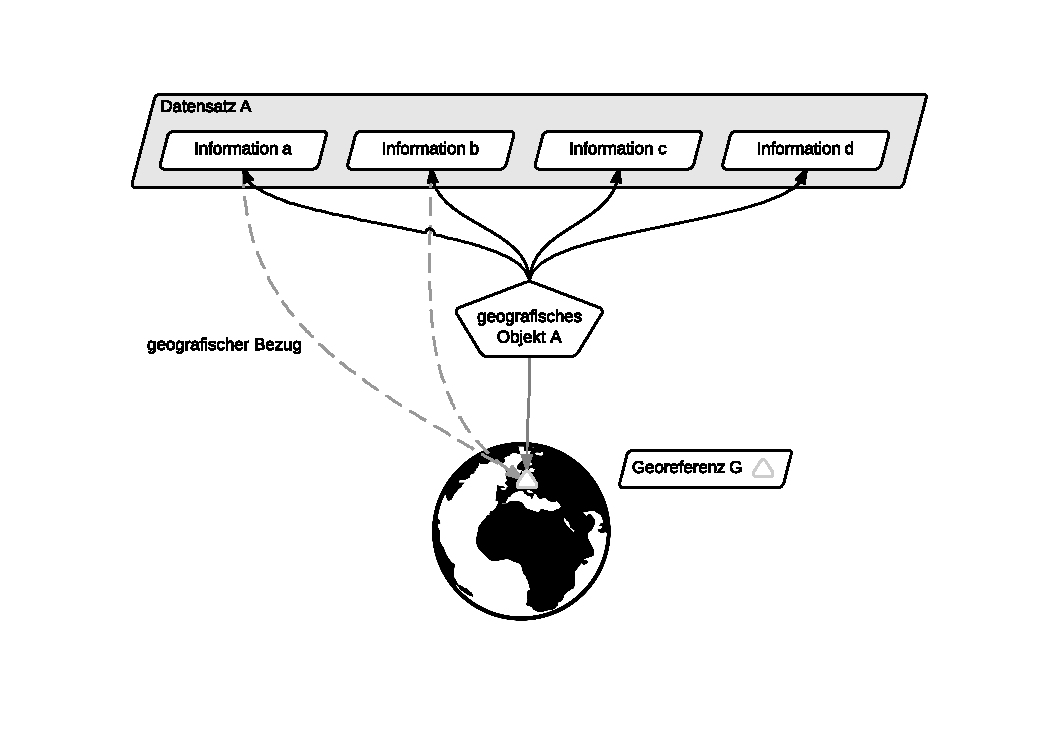
\includegraphics[scale=0.8]{geogIndikatoren.pdf}
				\caption{Geografische Indikatoren}
				\label{img:geogIndi}
			\end{center}
			\end{figure}	
			%Earth designed by Liane Thönnes from the thenounproject.com
			%Pin designed by Simple Icons from the thenounproject.com  

		\subsection{Geografische Hierarchie} \label{sub:geografischeHierarchie} 
			
			In der vorliegenden Arbeit wird eine geografische Hierarchie verwendet um eine Einteilung der Erde in geografische Regionen umzusetzen.

			Eine Aufteilung der Erde in geografische Regionen lässt sich auf oberster Ebene mit Hilfe von Ländern und deren Grenzen umsetzen. 
			Die meisten Länder sind in weitere administrative Einheiten aufgeteilt.
			Diese geografischen Regionen werden hier als Verwaltungseinheiten bezeichnet.
			Es wird zwischen Verwaltungseinheiten erster und zweiter Ordnung unterschieden. 
			Der Vatikan-Staat und das Fürstentum Monaco sind dabei Ausnahmen.
			Beide werden aufgrund ihrer Größe nicht in weitere Verwaltungseinheiten unterteilt.
			In der untersten Ebene der Hierarchie werden schließlich Städte dargestellt.


			Wenn man als Beispiel Deutschland heranzieht, ergibt sich eine Einteilung wie in Abbildung \ref{img:hierarchy} dargestellt. \footnote{Aus Platzgründen sind im Bild pro Ebene nur einige wenige geografische Objekte aufgezählt.} 
			Die oberste Ebene beschreibt das Land worauf die zweite Ebene die Bundesländer darstellt.
			Auf der dritten Ebene werden die Regierungsbezirke abgebildet, worauf die Städte in der letzten Ebene folgen. 
			Analog kann die Einteilung für die USA vorgenommen werden, woraus sich die Hierarchie Country->State->County->City ergibt.
			Jedes Objekt einer Hierarchieebene beschreibt eine geografische Region. 
			Insbesondere besteht in einer solchen Hierarchie eine Teilmengenbeziehung zwischen den Ebenen. 
			Ein Objekt in einer Ebene liegt immer innerhalb der ihm übergeordneten Objekte.
			Insbesondere liegt die geografische Region die ein Objekt beschreibt komplett innerhalb des ihm übergeordneten Objekts.			

			\begin{figure}[h!]
			\begin{center}
			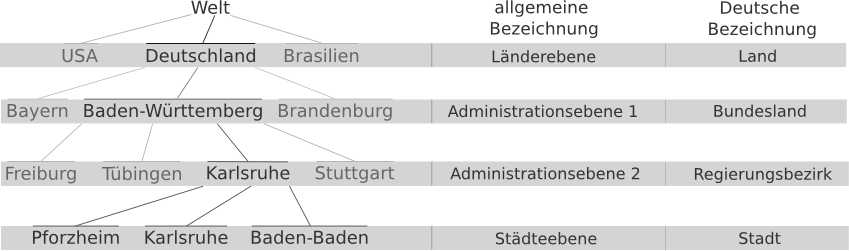
\includegraphics[scale=0.5]{hierarchie.png}
			\caption{Geografische Hierarchieebenen}
			\label{img:hierarchy}
			\end{center}
			\end{figure}	

			In Abbildung \ref{img:globusHierarchie} ist die Einteilung des Globus in Länder und Verwaltungseinheiten dargestellt. 

			\begin{figure}[h!]
			\begin{center}
			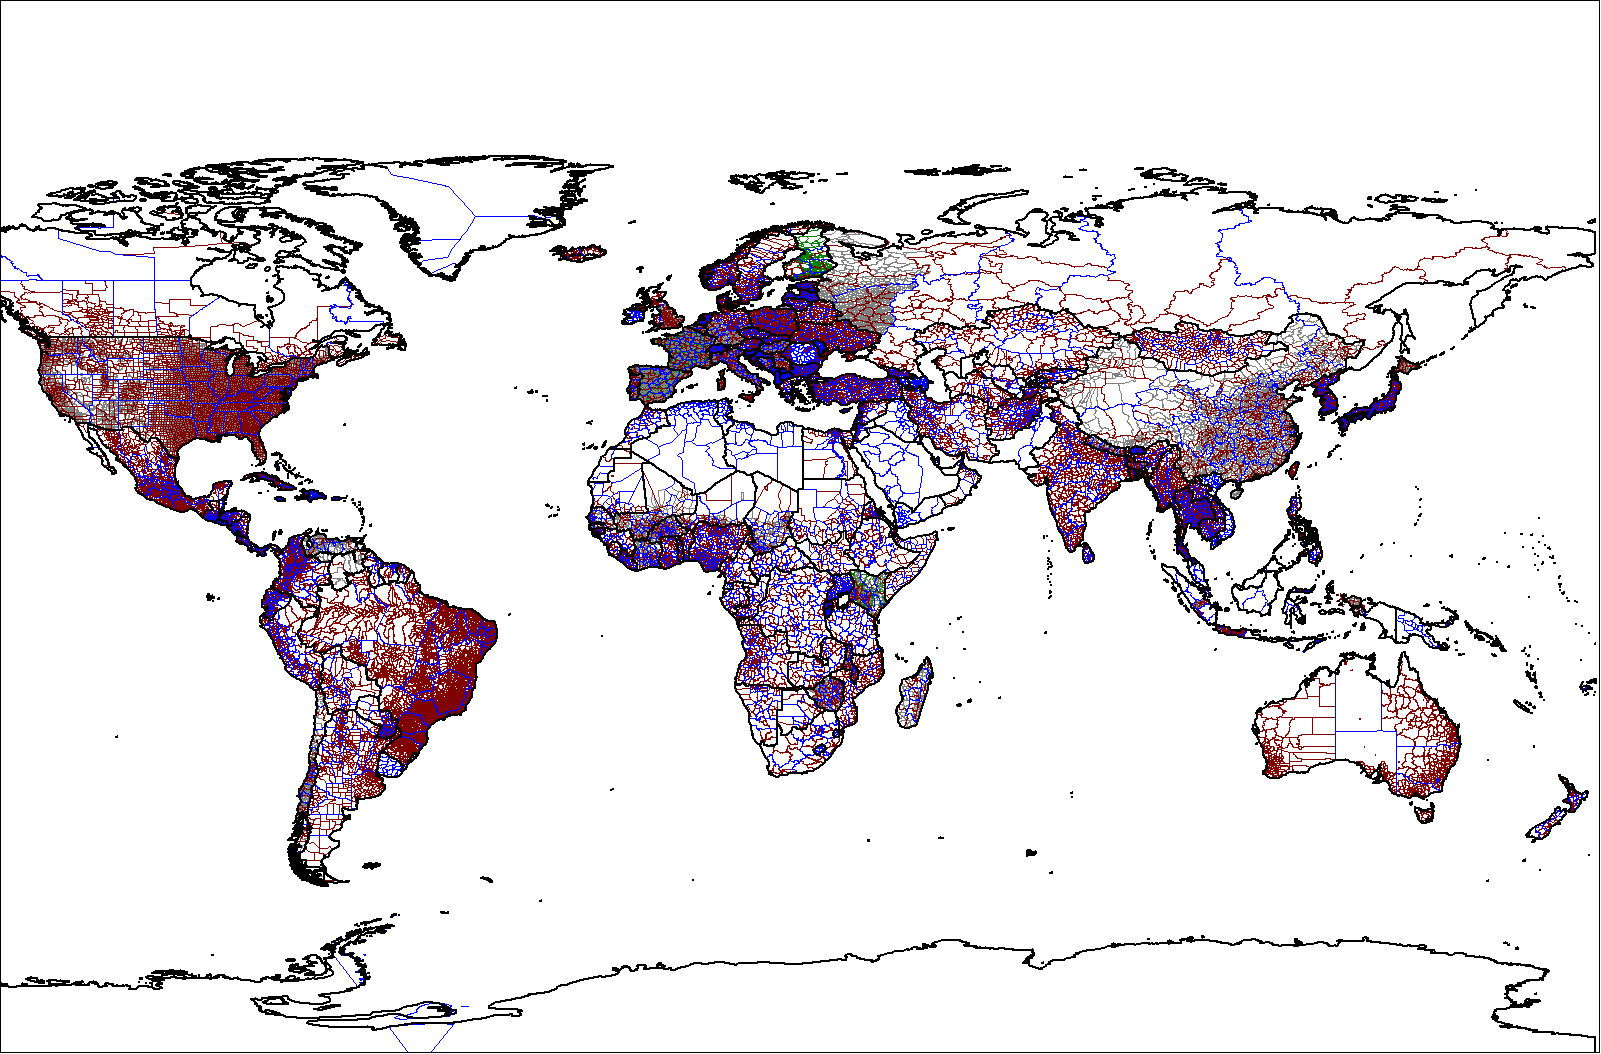
\includegraphics[scale=0.3]{globusHierarchie.png}
			\caption{Aufteilung der Welt in Verwaltungseinheiten}
			\label{img:globusHierarchie}
			\end{center}
			\end{figure}	
			%http://de.wikipedia.org/wiki/Verwaltungseinheit#mediaviewer/Datei:World_administrative_levels.png

		\subsection{Ortsverzeichnisse}

			In einem Ortsverzeichnis \footnote{Englisch: Gazetteer} sind Toponyme und deren zugehörige Georeferenzen gespeichert.
			Ortsverzeichnisse können sehr umfangreich sein und werden in Form einer Datenbank bereitgestellt.
			Meistens werden zu den Toponymen noch weitere Informationen hinterlegt.
			So bilden die Ortsverzeichnisse beispielsweise oft geografische Hierarchiebeziehungen ab.
			Aber auch Angaben zur Bevölkerungszahl oder die Angabe von alternativen Toponymen sind oft hinterlegt.

			Ortsverzeichnisse können genutzt werden um Toponymen eine Georeferenz zuzuweisen. 
			Dabei wird ein gegebenes Toponym im Ortsverzeichnis nachgeschlagen um die zugehörige Georeferenz zu erhalten.  

			\begin{description}

				\item[Geonames.org]
					
					Eines der bekanntesten Ortsverzeichnisse ist das frei erhältliche Ortsverzeichnis von geonames.org. 
					Dieses Ortsverzeichnis kann als CSV Datei\footnote{Comma Sperated Value} heruntergeladen werden.
					Neben umfangreichen Informationen wie Bevölkerungszahl, Sprache, Längen- und Breitengrad wird die geografische Hierarchie abgebildet.

					Die Daten von geonames.org werden aus diversen Quellen automatisch zusammengetragen. \footnote{Die genutzten Datenquellen können unter http://www.geonames.org/data-sources.html eingesehen werden} 
					Es werden allerdings auch Einträge von Nutzern erstellt. 
					Mittlerweile hat sich eine aktive Community rund um das Projekt entwickelt. 

					Das Ortsverzeichnis beinhaltet ca. 8,8 Millionen Toponyme und zugehörige Informationen. \footnote{Stand Dez. 2013, die Daten unterliegen ständiger Bearbeitung, die Anzahl der Einträge kann deshalb schwanken} 
					Hinzu kommen ca. 8 Millionen alternative Toponyme.
					Geonames.org ist damit eine der umfangreichsten frei erhältlichen Ortsverzeichnisse.

					Jedem Toponym ist eine geografische Position in Form von Längen- und Breitengrad zugeordnet. 
					Es wird allerdings kein Polygon zur Beschreibung der geografischen Region angegeben.
					Durch die Teilmengen Beziehung die in der geografischen Hierarchie abgebildet ist, können jedoch immer alle geografischen Hierarchieebenen bestimmt werden.

					In der vorliegenden Arbeit wird die geonames.org Datenbank mit Stand Dezember 2013 als Basis für geografische Informationen genutzt.
					Auch die verwendete geografische Hierarchie lässt sich aus der Datenbank gewinnen.

			\end{description}
			
		\subsection{Bestimmung der geografischen Hierarchieebenen zu einer geografischen Position} 
			
			Jede der geografischen Hierarchieebenen beschreibt eine geografische Region.
			Liegt eine geografische Position beispielsweise innerhalb der geografischen Region eines Landes soll das zugehörige Land bestimmt werden können.

			Im Ortsverzeichnis von geonames.org sind die geografischen Regionen allerdings nicht hinterlegt.
			Jedes geografische Objekt wird hier durch eine geografische Position beschrieben.
			Es kann zu einer geografischen Position also nicht direkt bestimmt werden in welcher geografischen Region diese liegt.

			Es soll nun ein Vorgehen vorgestellt werden, welches es trotzdem ermöglicht für eine beliebige geografische Position alle geografischen Hierarchieebenen zu bestimmen.
			
			\subsubsection{Verfahren zur Bestimmung der geografischen Hierarchieebenen}

				In der geografischen Hierarchie wird der Globus am genauesten durch die geografischen Regionen der Städte eingeteilt.
				Durch die Teilmengenbeziehung der geografischen Hierarchie sind mit der Stadt implizit alle anderen Hierarchieebenen bestimmt.

				Deshalb soll eine geografische Position der am nächsten liegenden Stadt zugeordnet werden.
				Dadurch wird der Globus auf Städteebene in geografische Regionen eingeteilt. 
				Eine geografische Region zu einer Stadt S umfasst dann genau die Fläche, innerhalb der keine andere Stadt näher liegt als S.

				Diese Flächen werden auch Voronoi-Regionen genannt.

			\subsubsection{Voronoi-Diagramme} 

				Sei eine Menge von Punkten $Z = {z_1,z_2,...,z_n}$ auf einer Ebene verteilt.
				Eine Voronoi-Region $V^i$ zu einem Punkt $z_i$ beinhaltet dann alle Punkte $P^i={p_1,p_2,...,p_n}$ die näher an $z_i$ liegen als an allen anderen Punkten $Z_j={z_j in Z|z_j!=z_i}$.
				Alle Voronoi-Regionen zu allen Punkten in Z bilden ein Voronoi-Diagramm.

				Dieses Konzept kann zur Bestimmung der nächstgelegenen Stadt verwendet werden. 
				Die geografischen Positionen der Städte bilden dabei die Punkte $Z$.
				Zu jeder Stadt wird nun die Voronoi-Region erzeugt. 
				Anhand der Voronoi-Region in der ein Punkt p liegt kann nun bestimmt werden welche Stadt am nächsten zu p liegt.

				Jeder Punkt auf dem Globus kann so einer Stadt zugeordnet werden.
				Insbesondere wird der Globus auf Städteebene in geografische Regionen eingeteilt.
				In Abbildung \ref{img:voronoi} ist ein Voronoi-Diagramm einiger deutscher Städte dargestellt.

				\begin{figure}[h!]
				\begin{center}
				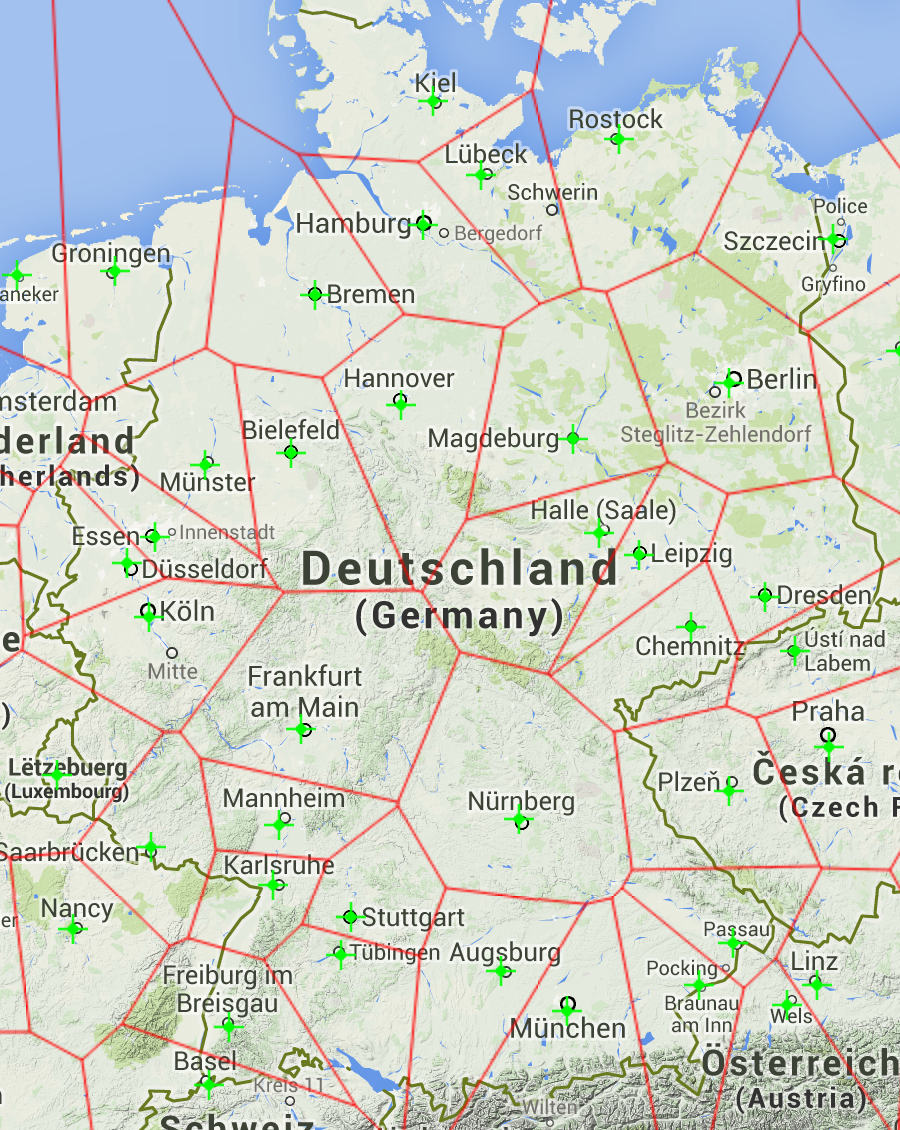
\includegraphics[scale=0.5]{voronoi.png}
				\caption{Vornoi-Diagramm Deutschland}
				\label{img:voronoi}
				\end{center}
				\end{figure}	

				Durch die Teilmengenbeziehung ist es nun nicht mehr nötig die geografischen Regionen der anderen Hierarchieebenen zu bestimmen.
				Es ist zu beachten, dass durch die Erzeugung der Vornoi-Regionen Ländergrenzen nur approximiert werden können. 
				Voronoi-Regionen zu Städten die in der Nähe einer Landesgrenze liegen können über die Landesgrenzen hinausgehen. 
				Damit werden geografische Positionen unter Umständen dem falschen Land zugeordnet.
				Auch dies ist in Abbildung \ref{img:voronoi} an den Landesgrenzen zu erkennen. 
				Umso größer allerdings die Anzahl der Städte ist, umso genauer wird die Approximation.

	\section{Toponyme in geografischen Indikatoren} \label{sec:ToponymeInGeografischenIndikatoren}

		In einem Datensatz zu einem geografischen Objekt können als Datenwerte Toponyme auftauchen.
		Toponyme eignen sich grundsätzlich gut als geografische Indikatoren.
		Sie geben den Namen eines geografischen Objekts an und haben unmittelbaren geografischen Bezug. 
		Mit Hilfe von Ortsverzeichnissen kann Toponymen eine Georeferenz zugeordnet werden.
		
		Bei der Verwendung von Toponymen als geografische Indikatoren können allerdings auch  Probleme auftreten.
		Toponyme sind nicht standardisiert.
		Es können dadurch beispielsweise mehrere Toponyme zu einem geografischen Objekt existieren.
		Es entsteht eine enorme Vielfalt an Toponymen. 
		Daneben können Toponyme auch Mehrdeutig sein.
		Das bedeutet: Ein Toponym kann sich auf zwei oder mehr unterschiedliche geografische Objekte beziehen.

		Im folgenden werden die Probleme genauer betrachtet.

		\subsection{Vielfalt der Toponyme}

			In Ortsverzeichnissen kann eine große Anzahl an Toponymen hinterlegt werden.
			Aufgrund der immensen Vielfalt an Toponymen ist es aber nahezu unmöglich alle existierenden Toponyme abzudecken. 

			Neben den offiziellen Namen für Städte, Länder usw. existieren eine Reihe von alternativen Toponymen.
			Auch Toponyme die spezielle geografische Objekte bezeichnen sind möglich.
			Grundsätzlich sind der Vielfalt von Toponymen keine Grenzen gesetzt.  

			Ein Beispiel für alternative Toponyme sind Spitznamen für Städte.
			In Wikipedia sind für die Stadt Detroit, im US-Bundesstaat Michigan, folgende Spitznamen angegeben: 

			 "'The Motor City"', "'Motown"', "'Hockeytown"', "'Rock City"', "'The D"'.

			Die ersten zwei dürften weltweit einen gewissen Bekanntheitsgrad haben. 
			"'Hockeytown"', "'Rock City"' und "'The D"' dürften allerdings weniger bekannt sein.
			Tatsächlich beinhaltet die geonames.org Datenbank keinen dieser Spitznamen.
			Durch eine Abfrage an dieses Ortsverzeichnis könnte somit keine Georeferenz bestimmt werden.
			Eine Abfrage in Google Maps hingegen bietet bei Eingabe der oben genannten Spitznamen Detroit als Vorschlag an. \footnote{http://de.wikipedia.org/wiki/Detroit (abgerufen Juli 2014)} 

		\subsection{Mehrdeutigkeiten von Toponymen} 

			Toponyme sind oft Doppel- oder Mehrdeutig und verweisen somit auf mehrere Georeferenzen.
			
			Es gibt zahlreiche Städte-Namen, die in mehreren Ländern verwendet werden.
			Ein gutes Beispiel hierfür sind US-Städte. 
			Da die USA ein Einwanderungsland ist, übernahmen viele Einwanderer bei der Gründung neuer Städte die Namen aus der alten Heimat. 
			So finden sich in den USA zahlreiche Städte deren Namen exakt den deutschen Städtenamen entsprechen. 
			In Tabelle \ref{tab:usCitiesGermanNames} sind einige Städte-Namen und die Vorkommen in den USA aufgelistet.
			
			\begin{table}[htpb]
				\caption{Häufige deutsche Städtenamen in den USA} 
				\centering
				\begin{tabular}{|c|c|}
					\hline
					Name & Anzahl in den USA \\
					\hline\hline
					Hannover & 40 \\
					\hline
					Berlin & 39 \\
					\hline
					Hamburg & 30 \\
					\hline
				\end{tabular}
				\label{tab:usCitiesGermanNames} 
			\end{table}

			Als Ergebnis einer Abfrage auf ein Ortsverzeichnis für das Toponym "'Hamburg"' würden 31 Georeferenzen in den USA und eine in Deutschland zurückgegeben werden. 

			Diese Mehrdeutigkeit stellt ein Problem dar.
			Es kann durch eine Abfrage an ein Ortsverzeichnis keine eindeutige Entscheidung getroffen werden welche Georeferenz dem Toponym zugewiesen werden soll. 

		\subsubsection{Fazit}

			Es existieren sehr umfangreiche Datenbasen um Toponymen eine Georeferenz zuzuweisen. 
			Toponyme unterliegen grundsätzlich keiner Kontrolle und sind nicht standardisiert womit der Vielfalt keine Grenzen gesetzt sind.
			Es ist schwer, wenn nicht sogar unmöglich, das Wissen über geografische Objekte und deren zugehörige Toponyme in Ortsverzeichnissen vollständig zu erfassen.


	


	\section{Twitter} 
	
		In diesem Kapitel werden grundlegende Begriffe rund um das Twitter-Netzwerk erläutert. 
		Weiter werden die Mechanismen in Twitter erläutert und an praktischen Beispielen erklärt. 
		Zum Schluss wird aufgezeigt welche Informationen pro Tweet übermittelt werden und welche Daten zur Lokalisierung verwendet werden können.

			\subsection{Geschichtliches}
			Twitter wurde 2006 von Jack Dorsey, Biz Stone, Noah Glass und Evan Williams gegründet.
			Ursprünglich war Twitter zur internen Kommunikation innerhalb der Firma Odeo geplant.
			Schnell wurde allerdings klar, dass in dem Dienst mehr potenzial steckt und so wurde Twitter öffentlich gemacht.
			Seitdem erfreut sich der Dienst einer wachsenden Nutzer-Gemeinde.
			Die Twitter-Gründer haben von Anfang an keine exakten Nutzer-Zahlen oder die Anzahl der versendeten Twitter-Kurznachrichten bekanntgegeben.
			Dies geschah einerseits, weil die Gründer davon überzeugt sind, dass anhand der reinen Nutzer-Zahlen und gesendeten Twitter-Kurznachrichten nicht die '"Gesundheit"' des Twitter-Netzwerks nachvollzogen werden kann, andererseits werden durch diese Massnahme auch strategische Ziele verfolgt.  \footnote{http://www.pbs.org/mediashift/2007/05/twitter-founders-thrive-on-micro-blogging-constraints137}
			2013 ging Twitter an die Börse und vermeldete 100 Millionen täglich aktive Nutzer und über 500 Millionen Twitter-Kurznachrichten, die täglich über den Dienst versendet werden. 

			\subsection{Was ist Twitter?}
			Twitter wird als Kurznachrichten-Dienst, Mikroblogging-Dienst oder auch als soziales-Netzwerk bezeichnet. 
			Twitter Geschäftsführer Kevin Thau hat 2010 auf dem Nokia-World Kongress öffentlich bestritten, dass Twitter ein Soziales-Netzwerk ist. 
			Laut Thau handelt es sich um ein Nachrichten-, Inhalts- und Informations-Netzwerk. 
			Er begründete dies damit, dass Twitter die Art und Weise wie Nachrichten verteilt werden geändert hat und praktisch jeder zum Journalisten werden kann. 
			Als Beispiel nennt er die Landung des Fluges 1549 auf dem Hudson River. 
			Die Augenzeugen hätten damals keine Mails versendet um die Nachricht zu verbreiten, sondern die Nachricht via Twitter weitergegeben.
			Es lassen sich eine Reihe weitere Beispiele derselben Art finden. 
			In \cite{Petrovic2013} wird ein Vergleich zwischen sogenannten Newswire anbietern und Twitter gezogen. \footnote{Newswire stellt eine Art Nachrichtenaggregator dar, über welchen Nachrichten aus verscheidenen Quellen aggregiert und weitergegeben werden. In deutschland kommt die Deutsche Presse agentur diesem Konzept am nächsten.}
			Es stellte sich heraus, dass über nahezu alle Nachrichten, welche in den Newswires verbreitet wurden auch im Twitter-Netzwerk berichtet wird.
			Nachrichten zu bestimmten, vermutlich sehr speziellen Themen oder Auslandsnachrichten wurden ausschliesslich in Twitter gefunden. 
			Diese Erkenntnisse decken sich mit der Einschätzung von Kevin Thau. 
			In \cite{Kwak2010} wird die Einschätzung, bei Twitter handele es sich nicht um ein soziales Netzwerk, wissenschaftlich bestätigt.
			Kwak et al überprüfen die in \cite{Newman2003} beschriebenen Eigenschaften sozialer Netzwerke und kommen zu dem Schluss, dass Twitter diese Eigenschaften nicht erfüllt.	

			Die Bezeichnung Kurznachrichten-Dienst ist irreführend, da dieser mit sms (small messeneger service) in Verbindung gebracht werden kann. 
			Tatsächlich galt der sms in der Anfangsphase von Twitter als Vorbild für den Dienst.
			In Twitter werden Nachrichten allerdings standardmäßig allen Benutzern zur Verfügung gestellt und können eingesehen werden. 
			Des weiteren wird eine Liste der Nachrichten, welche von einem Nutzer verfasst wurden, als Liste in umgekehrter chronologischer Reihenfolge auf dessen Profil dargestellt.
			Damit ähnelt das Twitter-Profil einem Blog mit Einträgen deren Länge 140 Zeichen nicht überschreiten darf. 
			Die Darstellung als Liste, und die Funktion einen Tweet standardmäßig allen Nutzern freizugeben unterscheidet sich grundlegend von der Funktion des sms, bei dem eine Nachricht direkt an einen Empfänger gesendet wird und nicht öffentlich ist.
			Im sms steht die Konversation zweier Nutzer im Vordergrund, wohingegen Nachrichten im Twitter-Netzwerk einen Brodcast an alle Nutzer darstellen.

			Die 140 Zeichen langen Nachrichten in Twitter werden als Tweets bezeichnet.
			Tweet bedeutet übersetzt Zwitschern, womit die Redenwendung '"Die Spatzen zwitschern es von den Dächern"' auch im Twitter-Netzwerk zu einer passenden Redenwendung  wird.  
			In der vorliegenden Arbeit wird Twitter deshalb als Mikroblogging-Dienst bezeichnet.
		

			\subsection{Funktionen von Twitter}
			Der Mikroblogging-Dienst Twitter bietet neben dem Profil, auf dem die Tweets des Nutzers angezeigt werden, noch eine Reihe weiterer Funktionen. 
			Im folgenden soll das Twitter-Profil und die Timeline kurz erläutert werden. 
			Eine der zentralen Funktionen von Twitter ist das sogennante Folgen, womit sich Nutzer win Netzwerk aufbauen können aus dem sie Twitter Nachrichten erhalten.
			Danach werden Funktionen wie das weitergeben eines Tweets, Favorisieren und Antworten erklärt. 
			Zum Schluss wird auf den gesendeten Tweet Inhalt eingenagen und der Netzwerk-Charakter von Twitter untersucht.

			\begin{figure}[h!]
			\begin{center}
			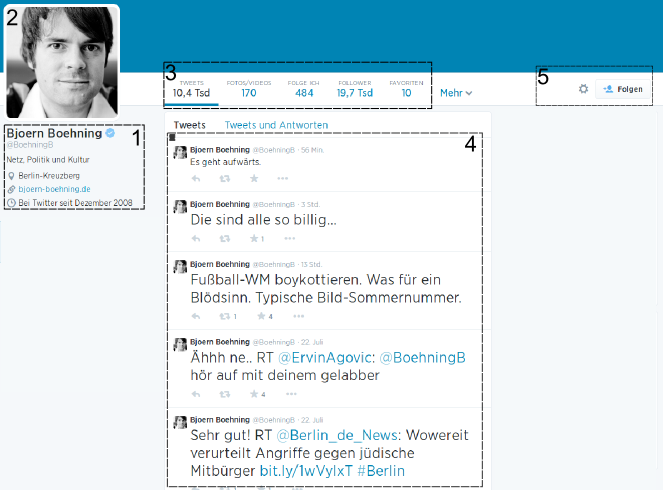
\includegraphics[scale=0.4]{profile.png}
			\caption{Die Twitter-Timeline auf einem Twitter Profil. 1: Nutzername und Informationen über den Nutzer. 2: Profilbild
			3: Allgemeine Informationen über den Benutzer und dessen Netzwerk
			4: Nutzer-Timeline: Tweets des Nutzer in umgekehrter chronologischer Reihenfolge 
			5: Button zum Folgen}
			\label{img:twitterProfile}
			\end{center}
			\end{figure}	


				\paragraph{Das Nutzer-Profil und die Nutzer-Timeline}
					Das Nutzer-Profil kann über die Url http://twitter.com/BENUTZERNAME abgerufen werden und bietet neben der Nutzer-Timeline, in der die Tweets des Nutzers angezeigt werden, eine Reihe an weiteren Informationen.
					In Abbildung \ref{img:twitterProfile} ist in der mitte die Timeline des Benutzers dargestellt in der dei Tweets zu sehen sind. 
					Unter dem Profilbild links sind Informationen des Nutzers aufgelistet.
					Diese Informationen kann der Nutzer selbst einstellen und entscheiden welche er angeben möchte.   


				\paragraph{Folgen (Following/Follower/Tweeps)}
					Diese Funktion erlaubt es Tweets eines bestimmten Nutzers zu abonnieren. 
					Im Twitter-Umfeld spricht man von '"following"' oder '"folgen"', wenn man die Tweets eines bestimmten Nutzers abonniert.
					Hat man Tweets eines bestimmten Nutzers abonniert so wird man als dessen '"Follower"' bezeichnet. 
					Das englische Wort '"Follower"' hat sich im Twitter-Umfeld und darüber hinaus eingebürgert und wird selten übersetzt. 
					Auch auf der Twitter Website wird '"Follower"' nicht ins deutsche übersetzt.
					In der vorliegenden Arbeit wird deshalb auch auf eine Übersetzung verzichtet. 

					In Abbildung \ref{img:twitterProfile} an Position 3 wird unter '"Folge ich"' die Anzahl der Twitter-Nutzer angezeigt denen der Beispielnutzer folgt. 
					Neben dem Feld '"Folge ich"' wird unter '"Follower"' angezeigt wieviele Nutzer dem Beispielnutzer folgen.

				\paragraph{Persönliche Timeline}
					Jeder Twitter-Nutzer hat seine persönliche Timeline, auf dieser werden die Tweets derjenigen Nutzer angezeigt, denen er folgt. 
					Die Timeline kann als Aggregation von Tweets betrachtet werden.
					Diese Timeline ist die zentrale Stelle, an der die Nutzer Tweets anderer Nutzer empfangen und lesen.
					Auch hier werden die Tweets in umgekehrter chronologischer Reihenfolge angezeigt.  

				\paragraph{Weiterleiten eines Tweets (Retweet)}
					Unter einem Retweet versteht man das weiterleiten eines Tweets den man nicht selbst verfasst hat an die eigenen Follower.
					Genauer gesagt wird der Tweet übernommen und ein Hinweis hinzugefügt, dass es sich um einen sogenannten Retweet handelt, und nicht einen vom Nutzer selbst verfassten Tweet.
					Diese Funktion wird hauptsächlich genutzt um Nachrichten schnell zu verbreiten ohne diese neu eingeben zu müssen. 
					Die Weitergabe an die eigenen Follower impliziert einen gewissen Grad an Kontrolle und Filterfunktion. 
					Der weitergebende Nutzer kontrolliert und filtert die Nachrichten die er erhält und gibt diejenigen weiter, denen er eine Gewisse Relevanz beimisst, oder von denen er erwartet, dass sie seine Follower interessieren. \todo{1 retweet Reichweite 1000 Nutzer}
					Mit dieser Funktion können einzelne Nutzer eine Art Filterfunktion übernehmen, welche früher Journalisten vorbehalten war. 
					Es darf jedoch nicht vergessen werden, dass der Nutzer nur im Rahmen seiner eigenen Möglichkeiten einen Tweet verifizieren kann und Nachrichten in Twitter keinesfalls gesicherte Fakten darstellen.
					Auch können Nutzer durch diese Funktion zu Tweet-Aggregatoren werden, welche Tweets von mehreren Nutzern erhalten oder sammeln, aber nur relevante oder themenspezifische Tweets weitergeben.

					\todo{Diagramm Retweet, Filterfunktion} 

				\paragraph{Hashtags}
					Hashtags werden genutzt um Tweet Nachrichten zu kategorisieren oder Metag Informationen zu liefern. 
					Ein Hashtag kann vom verfasser selbst als solches ausgezeichnet werden indem ein \# vor das gewünschte Wort, welches als Hashtag fungieren soll, gesetzt wird. 
					Hahstags ermöglichen es Tweets nach Stichworten zu filtern. 
					Anhand der Hashtags werden auch die Twitter-Trends analysiert.
					Twitter Trends 
					
				\paragraph{Antworten und direktes ansprechen eines Nutzers}
					Twitter bietet die Möglichkeit einzelne Nutzer direkt anzusprechen. 
					Mit Hilfe des @-Symbols kann ein Nutzer referenziert werden. 
					Der referenzierte Nutzer, besipielsweise @alfred, wird dann benachrichtigt, dass er in einem Tweet erwähnt wurde. 
					Der erwähnte Nutzer muss dabei nicht Follower des Verfassers sein. \todo{siehe Bild ref1} 
					Eine weitere Funktion im Twitter-Netzwerk ist das Antworten auf einen Tweet.
					Über eine Schaltfläche wird es ermöglicht auf einen Tweet zu Antworten. 
					Das @-Symbol und der Nutzername des Verfassers werden automatisch eingetragen, womit eine Benachrichtigung an den Verfasser des Ursprungstweets erfolgt. \todo{siehe Bild ref2}
					Es ist möglich, das auf einen Antwort-Tweet wiederum geantwortet wird, wodurch ein sogenannter Thread oder Konversation entsteht. \todo{siehe Bild ref3}
					Auch ist es möglich, dass an einer solchen Konversation mehrere Twitter-Nutzer beteiligt sind. 
					Dies ist dann der Fall, wenn im ursprünglichen Tweet, auf weitere User referenziert wurde. 
					Aber auch wenn ein Nutzer auf eine bestehende Konversation antwortet, werden alle beteiligtien Nutzer referenziert. \todo{siehe Bild ref4}
					\todo{Diagramm Antwort, Antwort Thread, Bild Antworten Button, Referenzieren}     


				\paragraph{Favorisieren}
					Mit dieser Funktion lässt sich ausdrücken, dass man einen Tweet interessant oder gut findet.
					Auch Zustimmung wird durch favorisieren ausgedrückt.  
					Einen Tweet zu favorisieren kann aber auch bedeuten '"ich habe deine Reaktion registriert"', oft um einen Antwort-Thread nicht abrupt abzubrechen sondern eine zustimmende Rückmeldung zu geben ohne extra einen Tweet zu verfassen.

			\subsection{Daten einer Twitter-Nachricht}
				Neben den direkt sichtbaren Informationen enthält ein Tweet eine Reihe weiterer Daten.
				Betrachtet man einen einzelnen Tweet, beispielsweise auf twitter.com, wird der Tweet-Text, der Verfasser und die Zeit, wann der Tweet verfasst wurde, mitgeteilt. \todo{siehe Bild} 
				Die Gesamtheit der Daten die in einem Tweet enthalten sind werden hier allgemein als Tweet-Daten bezeichnet.

				\begin{figure}[h!]
				\begin{center}
				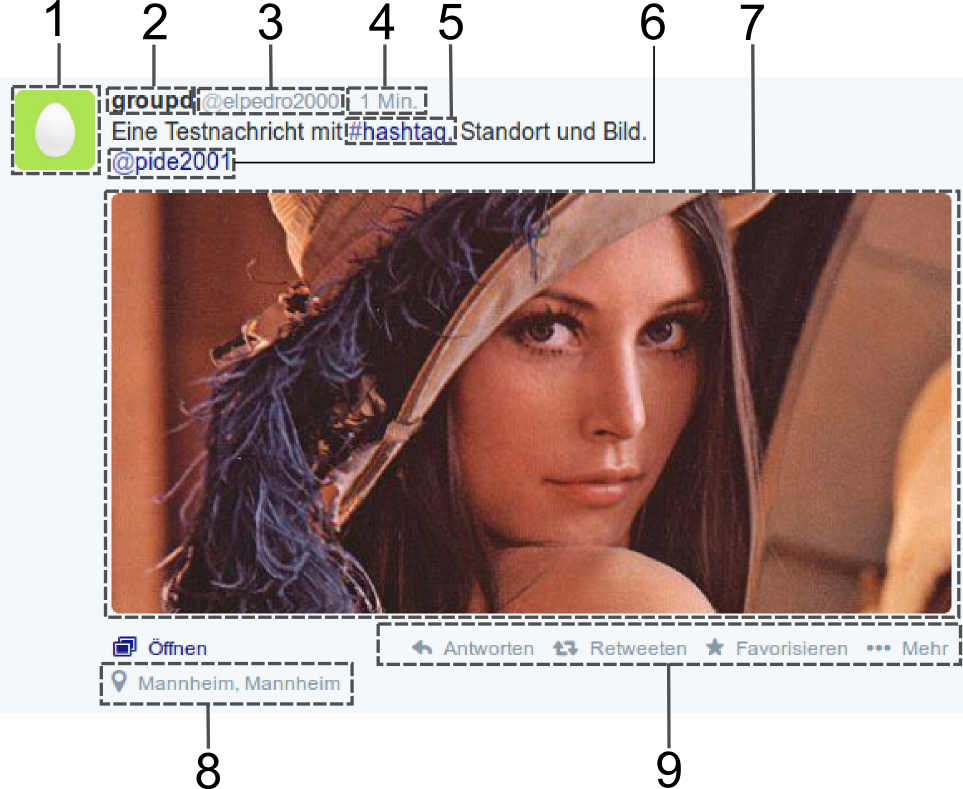
\includegraphics[scale=0.8]{tweetFinal.png}
				\caption{Was ist zu sehen?}
				\label{tweet}
				\end{center}
				\end{figure}	


				\paragraph{Koordinaten}
					In den Tweet-Daten können geografische Koordinaten in Form von Längen- und Breitengrad angegeben sein. 
					Diese Koordinaten zeigen an wo sich der Verfasser befand als er den Tweet abgesetzt hat.
					Wenn diese Koordinaten angegeben sind hat der Nutzer explizit zugestimmt, dass die Koordinaten seines aktuellen Aufenthaltsortes dem Tweet angehängt werden. 
					Die Bestimmung der Koordinaten und das anhängen der Koordinaten an einen Tweet werden vollautomatisch durch das Programm übernommen mit welchem der Tweet verfasst wurde.
					Auf Smartphones wird meist das integrierte GPS-Modul genutzt um die Koordinaten zu bestimmen. 
					Bei der Nutzung an einem PC wird der Tweet häufig über den Browser verfasst und die Position mit Hilfe von GeoIp ermittelt.


			 	\paragraph{Daten}
			 		Neben den sichtbaren Daten, welche in der Timeline angezeigt werden, enthält ein Tweet eine Reihe weiterer interessanter Informationen. 	


			

		 	\subsection{Geoinformationen in Twitter Daten}
		 		\todo{Überarbeiten subsec:Geoninformationen in Twitter Daten} 
		 		\subsubsection{Welche Tweet-Daten können zur Georeferenzierung herangezogen werden} \todo{Nur optional} 

					Um diese Frage zu beantworten, müssen die Tweet-Daten eingehend untersucht werden. 
					Dabei spielt nicht nur die reine Information die den Daten entnommen werden kann eine Rolle, sondern auch wie die Daten generietr oder eingegeben wurden.
					Beispielsweise kann bei einem Tweet, dem ein Längen- und Breitengrad mit einer Genauigkeit von 14 Nachkommastellen zugeordnet ist, davon ausgegangen werden, dass die geografische Position der tatsächlichen geografischen Position, von welcher der Tweet abgesetzt wurde, entspricht. 
					Es liegt hier die Vermutung nahe, dass diese Werte durch ein mobiles GPS \footnote{Global Positioning System} erfasst worden sind. 
					Anders verhält sich dies beispielsweise beim Tweet-Text, eine Erwähnung der Stadt New York, muss nicht bedeuten, dass der Tweet aus dieser Stadt stammt. 
					Es impliziert nicht einmal, dass der Verfasser jemals in dieser Stadt war.  
					Im folgenden werden einige Datenfelder, welche mit jedem Tweet versandt werden, untersucht.
					Dabei wird die Eignung dieser Daten als geografischer Indikatoren bewertet.
					Währenddessen werden anhand geeigneter Beispiele die Bergiffe gesicherter -, ungesicherter -, mittelbarer - und unmittelbarer geografischer Indikator eingeführt.  

				\subsubsection{mögliche geografische Indikatoren} 

					\paragraph{Nutzer-Standort} 
						
						Der Nutzer-Standort ist ein unmittelbarer geografischer Indikator.  
						Als Nutzer-Standort kann der Twitter-Nutzer eine beliebige Zeichenfolge eingeben. 
						Es handelt sich beim Nutzer-Standort deshalb um einen ungesicherten geografischen Indikator, es ist deshalb damit zu rechnen, dass unter Umständen keine geografische Position angegeben ist und andererseits keine einheitliche Angabe bezüglich des selben Standorts erwartet werden kann.
						Beispielsweise beschreiben die Zeichenketten "'Karlsruhe, Deutschland"' und "'Baden-Württemberg, Karlsruhe"' den selben Ort.
						Noch deutlicher wird dieser Umstand, wenn man alternative Namen oder umgangssprachliche Namen für Städte betrachtet. 
						Mit "'The Big Apple"' und "'New York, USA"' oder mit "'Motown"' und "'Detroit, MI"' sind dieselben Orte gemeint.   
						Auch die Genauigkeit bezüglich der geografischen Position ist nicht zuverlässig vorhersagbar, sehr konkrete geografische Positionen, wie die Angabe einer Stadt oder eines Stadtteils, oder aber eine geografische Region wie beispielsweise ein Land oder ein Kontinent, sind möglich. 


					\paragraph{Nutzer-Zeitzone} 

						Die Nutzer-Zeitzone stellt dagegen einen gesicherten, unmittelbaren geografischen Indikator dar.
						Bei der Nutzer-Zeitzone kann aus einer Liste möglicher Werte gewählt werden, womit keine Ungenauigkeiten bezüglich der Eingabe besteht und eine definierte Zeichenkette erwartete werden kann, deren geografische Region klar definiert ist. 
						Die Nutzer-Zeitzone beschreibt allerdings in jedem Fall eine größere geografische Region, die nicht immer mit den konventionellen Ländergrenzen korrespondiert und somit eine Bestimmung der geografischen Position nahezu unmöglich macht.
						\todo{Irgendwo auf den Umstand eingehen, dass Timezone nicht angegeben werden wird und dann der Standard gewählt wird der us central pacific time ist? .......} 

						Bei beiden Indikatoren besteht natürlich die Möglichkeit der Falscheingabe durch den Benutzer. Dieser Umstand wird jedoch durch die Analyse der Daten ausgemerzt. \todo{Umschreiben und woanders darauf eingehen!} 

	
		

			
\chapter{Stand der Technik} 
	Die Georeferenzierung von Tweets oder Twitter-Nutzern ist ein Feld an dem nach wie vor aktiv geforscht wird.
	Nicht zuletzt trägt auch die große Verfügbarkeit an Twitter-Daten zu dem Umstand bei, dass Twitter in den letzten Jahren Forschungsgegenstand zahlreicher Publikationen war. 
	
	In diesem Abschnitt sollen bestehende Ansätze zur Georeferenzierung im Twitter-Umfeld untersucht werden. 
	Es werden Kriterien zur Einordnung der bestehenden Ansätze erarbeitet und erläutert.   
	Die Arbeiten werden mit Hilfe der Kriterien schematisch eingeordnet um einen Überblick zu erhalten. 
	Zum Schluss wird untersucht ob die Arbeiten die bereits formulierten Anforderungen aus \ref{sec:Anforderungen} erfüllen, und wie sich die vorliegende Arbeit von den bestehenden Ansätzen abgrenzt.    

		\section{Kategorisierung bestehender Ansätze}

		In früheren Arbeiten wurde bereits versucht, eine Einordnung der bestehenden Verfahren vorzunehmen. 
		Es ist interessant die Kategoriesierungsansätze und die verwandten Arbeiten einiger Autoren zu studieren.
		Es lässt sich dadurch die Entwicklung zum Thema Lokalisierung im Twitter-Umfeld beobachten. 
		Einige Kategorisierungsansätze werden im folgenden aufgelistet und erläutert.

		Sowohl in \cite{Hecht2011} als in \cite{Cheng2010} beschränken sich die verwandten Arbeiten nicht auf die Lokalisierung im Twitter-Umfeld, es werden Arbeiten zur Lokalisierung von Web-Inhalten im Allgemeinen aufgelistet. 
		Dies lässt darauf schliessen, dass sich vor den Jahren 2010/2011 nur wenige Arbeiten mit der Lokalisierung im Twitter-Umfeld beschäftigt haben.  
		
		\subsubsection{Kategorisierung über die untersuchte Ressource}
		\cite{Hecht2011} nimmt deshalb eine Kategorisierung anhand der untersuchten Ressource vor. 
		Es wird unterschieden zwischen Forschungen zur "'Lokalisierung von Microblogging-Seiten und deren Inhalten"' und der "'Lokalisierung von Nutzern, welche Inhalte zu Web 2.0 Seiten beisteuern"'. 
		Zusätzlich wird in dieser Arbeit das "'Verhalten der Nutzer im Umgang mit der Veröffentlichung ihres aktuellen Standorts"' und die "'Vorhersage privater Informationen"' betrachtet. Darauf soll hier allerdings nicht weiter eingegangen werden.      

		\subsubsection{Kategorisierung über die verwendete Methode}

		\cite{Cheng2010} klassifiziert die vorgestellten Arbeiten anhand der verwendeteten Methodik. 
		Es wird auf Arbeiten zur Lokalisierung von Webseiten, Web-Logs, Suchanfragen und Web-Nutzern verwiesen. 
		Diese werden in die folgenden drei Kategorien eingeteilt.

		\paragraph*{"'Inhaltsanalyse mit Begriffen in einem geografischen Verzeichnis (Content analysis with terms in a gazetteer)"'}  
		Es wird darunter eine einfache Datenbanksuche verstanden. 
		Es werden einzelne Wörter in einer Datenbank nachgeschlagen um diese einem konkreten geografischen Ort zuweisen zu können.
		Dabei kann sowohl lokal auf eine Geo-Datenbank als auch auf Internet Ressourcen zurückgegriffen werden.  
		In der Regel durchläuft der untersuchte Text eine manuelle oder automatische Vorverarbeitung um potenziell geografische Begriffe, sogenannte Toponyme, herauszufiltern. 

		\paragraph*{"'Inhaltsanalyse mit probabilistischen Sprachmodellen (Content analysis with probabilistic language models)"'}
		Dabei werden Texte oder Textteile einer Twitter-Kurznachricht zu vordefinierten geografischen Regionen wie Ländern oder Städten zugeordnet. 
		Nach einer Vorverarbeitung des Textes erfolgt eine statistische Auswertung, um danach den Text oder einzelne Textteile, wie beispielsweise Wörter, einer geografischen Region zuzuordnen. 
		Eine unbekannter Text kann dann mit Hilfe der zuvor gelernten Zuordnung einer geografischen Region zugeordnet werden.

		\paragraph*{"'Schlussfolgerungen durch soziale Verbindungen (Inference via social relations)"'} es werden soziale Verbindungen, die in Netzwerken abgebildet sind, herangezogen um Rückschlüsse auf den geografischen Ort des untersuchten Inhaltes oder einer Person ziehen zu können.

		Preidhorsky et al. schlagen in \cite{Priedhorsky2013} eine weitere Einteilung anhand der Methodik vor. 
		Allerdings werden hier ausschließlich Arbeiten im Twitter-Umfeld betrachtet. 

		\paragraph*{"'Geocoding"'} Im wesentlichen entspricht dies der "'Inhaltsanalyse mit Begriffen in einem geografischen Verzeichnis"' aus \cite{Cheng2010}. 
		"'Geocoding"' wird als Begriff in vielen Fachrichtungen unterschiedlich definiert, was zu Missverständnissen führen kann. 
		In \cite{bibsmaniaaa:Goldberg2008} wird genauer auf den Begriff des Geocoding und die Poblematik eingegangen und eine Definition  des Begriffs vorgeschlagen.
		Im vorliegenden Kontext ist es präziser und weniger missverständlich die Methodik als "'Inhaltsanalyse mit Begriffen in einem geografischen Verzeichnis"' zu bezeichnen, anstatt den Begriff "'Geocoding"' einzusetzen. 
		
		\paragraph*{"'Geografische Themenmodelle (geografic Topic Modeling)"'} wird definiert als die Verbindung von "'Themenmodellierung"' und "'Standorterkennung (Location Awareness)"'. 
		Durch klassisches "'Themenmodellierung"' lässt sich aus aus Texten eine Menge von Themen extrahieren. 
		Durch eine Lernphase werden Wörterbücher zu den Themen erstellt.
		Mit Hilfe dieser Themen-Wörterbücher kann später das Thema eines Textes bestimmt werden. \cite{Blei2012} 
		Unter "'Standorterkennung"' wird hier verstanden, dass nicht nur das Thema sondern auch eine bestimmte Region extrahiert werden kann. 
		Dies kann durch geografischen Koordinaten in Twitter-Kurznachrichten realisiert werden. 
		Im Unterschied zur Kategorie "'Inhaltsanalyse mit probabilsitischen Sprachmodellen"' aus \cite{Cheng2010} wird hier jedoch keine vorgegebene geografische Region gefordert. 
		Vielmehr ergeben sich die geografischen Regionen aus den Themenmodellen und den zugehörigen geografischen Koordinaten.
		Es wird damit eine kontinuierliche Region beschrieben, welche nicht zwangsweise durch Stadt-, Staaten- oder Ländergrenzen beschränkt ist.  

		\paragraph*{"'Statistische Klassifizierung (Statistical classifiers)"'} Diese Kategorie entspricht der "'Inhaltsanalyse mit probabilsitischen Sprachmodellen"' wobei in \cite{Cheng2010} nur eine Arbeit in dieser Kategorie betrachtet wird. \cite{Priedhorsky2013} listet mehrere Arbeiten auf, die sich in diese Kategorie einordnen lassen.   

		\paragraph*{"'Informationen aus sozialen Verbindungen (Social Network Information)"'} analog zu "'Schlussfolgerungen durch soziale Verbindungen"' aus \cite{Cheng2010} werden soziale Verbindungen herangezogen um den Standort zu bestimmen. 

		Priedhorsky et al. wählen eine ähnliche Einteilung wie vormals Cheng et al. in 2010, die verwandten Arbeiten stammen allerdings aus dem Twitter-Umfeld. 
		Dabei ist zu bemerken, dass sich die verwendeten Methoden zur Lokalisierung im Twitter-Umfeld nicht wesentlich von denen in anderen Bereichen unterscheiden. 
		Um die Arbeiten im Twitter-Umfeld sinnvoll voneinander abgrenzen zu können muss die Kategorisierung mehr Dimensionen umfassen. 
		Es müssen mehr Kriterien zur Kategorisierung herangezogen werden als die reine Methodik.   

		Mahmud et al. betrachten in \cite{Mahmud2012} hauptsächlich Arbeiten im Twitter-Umfeld. 
		Diese werden in die folgenden Kategorien unterteilt. 

		\begin{enumerate}
			\item  "'Inhaltsbasierte Standortschätzung von Tweets (Content-based Location Estimation from Tweets)"'
			\item "'Inhaltsbasierte Standortextrahierung von Tweets (Conetnt-based Location Extraction from Tweets"'
			\item "'Standortschätzung ohne den Tweet Inhalt zu nutzen (Location Estimation without using Tweets Content)"'
		\end{enumerate}

		\paragraph*{"'Inhaltsbasierte Standort-Schätzung von Tweets (Content-based Location Estimation from Tweets)"'} hier wird die geografische Position durch eine Inhaltsanalyse der Twitter-Kurznachricht geschätzt. 
		Die Schätzung erfolgt dabei durch probabilistische Modelle.
		Diese Kategorie vereint damit "'Geografische Themenmodelle"', "'Statistische Klassifizierung"' aus \cite{Priedhorsky2013} mit "'Inhaltsanalyse mit probabilsitischen Sprachmodellen"' aus \cite{Cheng2010} und ist damit als genereller anzusehen, als die vorgenannten Kategorien. 

		\paragraph*{"'Inhaltsbasierte Standort-Extrahierung von Tweets (Content-based Location Extraction from Tweets"'} die verwandten Arbeiten in dieser Kategorie versuchen direkte Hinweise auf einen geografischen Ort aus einer Twitter-Kurznachricht zu extrahieren. 
		Diese Kategorie ähnelt dem "'Geocoding"' beziehungsweise der "'Inhaltsanalyse mit Begriffen in einem geografischen Verzeichnis"'. 

		\paragraph*{"'Standortschätzung ohne den Tweet Inhalt zu nutzen (Location Estimation without using Tweets Content)"'} hierunter versteht der Autor alle Informationen die nicht unmittelbar im Tweet-Text enthalten sind. Dazu zählen Informationen aus dem Nutzerprofil oder Informationen über die sozialen Verbindungen des Nutzers.


		\cite{Mahmud2012} nutzt ebenfalls die Methodik um die Arbeiten zu kategorisieren. 
		Allerdings wird hier eine generellere Einteilung vorgenommen. 
		So wird unterteilt, ob der Standort geschätzt oder extrahiert wurde.  
		Mahmud et al. bringen aber auch eine weitere Dimension ein. 
		Es wird hier zusätzlich unterschieden ob das angewendete Verfahren den Tweet-Inhalt nutzt oder andere Informationen. 

		Dies ist sinnvoll, denn die genannten Methoden lassen sich sowohl auf den Tweet-Inhalt als auch auf andere Informationen, beispielsweise aus dem Nutzerprofil, anwenden. 
		
		Frühere Arbeiten verweisen auf ein weiteres Spektrum an Arbeiten aus anderen Bereichen, wie Lokalisierung von Flickr Bildern oder Web-Log Einträgen.
		Arbeiten zur Lokalisierung im Twitter-Umfeld werden hier seltener erwähnt. 
		In späteren Arbeiten, wie in \cite{Priedhorsky2013}, wird hingegen fast ausschließlich auf Arbeiten aus dem Twitter-Umfeld verwiesen. 
		Dies spiegelt die steigende Anzahl der Arbeiten zur Lokalisierung im Twitter-Umfeld wieder.
		Betrachtet man die Ausarbeitungen zur Lokalisierung im Twitter-Umfeld genauer, wird allerdings schnell klar, dass die Kategorisierung der Arbeiten anhand der verwendeten Methodik, dem Umfang nicht mehr gerecht wird. 
		
		Bei genauerer Betrachtung der Arbeiten stellt man allerdings fest, dass diese Klassifizierungen dem Umfang der Arbeiten nicht gerecht wird. 
		\cite{Hecht2011} verweist auf ähnliche Ansätze mit einem anderen Untersuchungsgegenstand.
		\cite{Cheng2010} kategorisiert die Arbeiten anhand der Methodik, und verweist ebenso auf andere Untersuchungsgegenstände. 
		\cite{Priedhorsky2013} verweist ausschliesslich auf Arbeiten im Twitter-Umfeld und kategorisiert diese anhand der verwendeten Methodik. 
		Die Methodeneinteilung ist aufgrund der Begriffswahl missverständlich und kann somit zu Problemen führen. 

		\subsection{ttt<sss}
		In \cite{Schulz2013} werden die folgenden Dimensionen zur Abgrenzung herangezogen.

		\todo{Indikatoren aus \cite{Schulz2013}}

		Allerdings lassen sich noch andere Dimensionen zur Klassifizierung der Arbeiten heranziehen. 
		Wird besipielsweise der Text einer Twitter-Kurznachricht durch eine einfache Geokodierung untersucht wird dies andere Ergebnisse liefern als eine Untersuchung auf Basis eines geografischen Themenmodells.  
		

		\cite{Hecht2011} nutzen diese Methode um eine Ground-Truth zu bestimmen indem das Userlocation-Feld in Wikipedia nachschlagen wird. Wikipedia bietet zu vielen Artikeln eine grografische Position in Form von Längen- und Breitengrad an, diese werden dann der untersuchten Twitter-Kurznachricht zugeordnet. 
		\cite{Hale2012} nutzen die Yahoo und die Google Geocoding Api um das Userlocation-Feld eingehender zu untersuchen.  
		

		
		Eine weitere zu betrachtende Dimension stellt daher der konkrete Untersuchungsgegenstand in Form des Indikators dar.


		Betrachtet man die Gesamtheit an arbeiten im Bereich der Lokalisierung im Twitter Netzwerk drängen sich noch mehr Dimensionen zur Klassifizeirung der arbeiten auf.

		\begin{enumerate}
		 	\item Räumliche Indikatoren
		 	\item Techniken
		 	\item Fokus der Lokalisierung
		 \end{enumerate} 	


		\todo{Tabelle einfügen, bereits fertig, nur noch Format anpassen (Lesbarkeit)}
		\todo{Requirements Tabelle einfügen}

		

		\begin{enumerate}
			\item Naiver Ansatz -> Geocoding mit Google Maps API V3, nur Indikatoren die geografische Namen enthalten. 
					Prinzipiell einfache Datenbankabfrage mit ein wenig semantik. 
					Keine Jargon Namen wie Big Apple etc.
				\begin{enumerate}
					\item Funktion der GMaps Api V3
					\item Einschränkungen der GMaps Api V3
					\item zurückgelieferte Daten der GMaps Api V3
					\item Kurze Beschreibung wie ich die API genutzt habe
				\end{enumerate}
			\item aktuelle Ansätze
				\begin{enumerate}
					\item Verfahren mit Inhaltsanalysen
					\item Verfahren mit Indikatoren einzelne oder mehrere
					\item Welche Verfahren kommen beim mapping auf \todo{geografische Entität definieren} geografische Entitäten zum Einsatz
				\end{enumerate}
		\end{enumerate}

		\subsection{Probleme früherer Ansätze}
			\begin{enumerate}
				\item{Genutzte API's und Indikatoren nur in bestimmten Sprachen verfügbar}
				\item{keine Schätzung für Genauigkeit auf verschiedenen geografischen Hierarchieebenen verfügbar}  
			\end{enumerate}

	
	
	

	
